%!TEX root = ../../thesis.tex

ggF is modelled by \meps{\powhegbox}{\pythia{8}}, including the exact mass 
dependence of the \Ptop and \Pbottom quarks in the loop \cite{Powheg-ggF-quarkmasses}. 
The CT10 PDF \cite{CTEQ} was used to model the incoming partons.
The \powhegbox parameter \verb|hfact| controls the scale at which the emission 
transitions from Sudakov-like to ME-like. This is tuned to $\mH/1.2$ in order to 
reproduce the Higgs boson \pt distribution of \hqt \cite{HqT2} (NLO+NNLL accuracy). This 
tuning is further discussed in \Section~4.9 of \Reference \cite{YR2}.



\subsection{Higgs boson transverse momentum}
\label{sec:ggF:pt}
\todo[inline]{Include Higgs \pt studies?}



\subsection{Event selection acceptance}
\label{sec:ggF:acc}

In \Section~\ref{sec:ggf_jetbin}, perturbative uncertainties in the jet binning were 
considered. We now consider uncertainties in the acceptance of the event selection. These 
are evaluated at hadron-level (\ie before detector simulation) by changing some aspect of 
the MC modelling and measuring the effect upon the acceptance within each jet bin. 
The selection criteria are similar to those applied at detector-level (see 
\Table~\ref{tab:signal:acc_truthselection}).

Hadron-level object definitions follow. The MC event record is used to identify leptons 
and neutrinos which descend from the Higgs boson. An \metvec vector is constructed from 
the neutrinos. Each lepton is `dressed' with the four-momenta of photons within a cone of 
$\Delta R < 0.1$, in order to recover energy lost via QED FSR. Jets are found using 
individual particles as inputs (\cf topo-clusters at detector-level). Muons and neutrinos 
are excluded from jet finding since they interact weakly with the calorimeter. Objects 
must pass the same \pt, $\eta$ and overlap removal criteria applied at detector-level.

\begin{table}
	\begin{tabular}{ccc}
		\toprule
		Jet binning & \emch/\mech & \eech/\mmch \\
		\midrule
		Inclusive & \multicolumn{2}{c}{$\ptleadlep > 22$ and $\ptsubleadlep > 10$} \\
		& $\mll > 10$ & $\mll > 12$ \\
		& -- & $\mods{\mll - \mZ} > 15$ \\
		& $\met > 20$ & $\metrel > 40$ \\
		& \multicolumn{2}{c}{$\mll < 55$} \\
		& \multicolumn{2}{c}{$\dphill < 1.8$} \\
		\midrule
		0-jet & \multicolumn{2}{c}{$\dphillmet > \pi/2$} \\
		& \multicolumn{2}{c}{$\ptll > 30$} \\
		\midrule
		1-jet & $\maxmtw > 50$ & -- \\
		& $\mtautau < \mZ - 25$ & -- \\
		\midrule
		\twojet & $\mtautau < \mZ - 25$ & -- \\
		& \multicolumn{2}{c}{Fail $\dyjj > 3.6$ or $\mjj > 600$ or CJV or OLV} \\
		\bottomrule
	\end{tabular}
	\caption{Hadron-level event selection used to calculate ggF acceptance uncertainties. 
	Cuts on energy, momentum and mass are given in \GeV, and angular cuts are given in 
	radians. The CJV and OLV are the central jet veto and outside lepton veto, 
	respectively. See \Chapter~\ref{chap:selection} for a detailed explanation of the 
	criteria.}
	\label{tab:signal:acc_truthselection}
\end{table}

Four sources of theoretical uncertainty are considered:
\begin{itemize}[noitemsep,nolistsep]
	\item higher order corrections,
	\item PDFs,
	\item parton shower, hadronisation and underlying event models,
	\item NLO-PS matching scheme.
\end{itemize}

Uncertainties due to higher order corrections are evaluated via independent variation of 
renormalisation and factorisation scales in the range $\mH/2 \leq \mur,\muf \leq 2\mH$, 
whilst observing the constraint $1/2 \leq \mur/\muf \leq 2$. In the \twojet bin, scale 
uncertainties are evaluated \todo{H+2j scale uncertainties in acceptance} with \mcfm 
\cite{MCFM:H2j}. This is necessary because \powhegbox is an NLO generator and therefore 
cannot probe perturbative uncertainties in the \twojet bin.

Uncertainties due to PDFs are evaluated in two ways. The acceptance is compared to 
that predicted with the MSTW2008 PDF \cite{MSTW}. Also, the set of PDF eigenvectors 
corresponding to 90\% CL of the CT10 fit were used to evaluate an uncertainty, 
which was then rescaled to 68\% CL. PDF uncertainties are calculated relative to the 
inclusive cross section, in order to include uncertainties in the jet binning. These are 
evaluated using \mcatnlo.

Uncertainties due to the parton shower (PS), hadronisation and underlying event (UE) 
models are evaluated by comparing \powhegbox showered by \pythia{8} (nominal), \pythia{6} 
and \fherwig. Uncertainties due to the NLO-PS matching scheme are evaluated by comparing 
\meps{\powhegbox}{\fherwig} to \meps{\mcatnlo}{\herwigpp}.

The acceptance uncertainties for each signal region used in the fitting procedure are 
shown in \Table~\ref{tab:signal:acc_unc}.

\begin{table}
	\centering
	\begin{tabular}{ccc|cccccc}
		\toprule
		& \mll & \ptsubleadlep & \multirow{2}{*}{Scale} & \multicolumn{2}{c}{PDF} & \multicolumn{2}{c}{PS/UE} & \multirow{2}{*}{NLO-PS} \\
		& (\GeV) & (\GeV) & & collab. & 68\% CL & \pythia{6} & \fherwig & \\
		\midrule
		\multicolumn{9}{c}{\eech/\mmch channels} \\
		\midrule
		0-jet & 12--55 & $>10$ & 1.4\% & +1.9\% & 3.2\% &   $+1.6\%$ & $+6.4\%$ &   $-2.5\%$ \\
		1-jet & 12--55 & $>10$ & 1.9\% & +1.8\% & 2.8\% & $(-)1.5\%$ & $+2.1\%$ & $(-)1.4\%$ \\
		\midrule
		\multicolumn{9}{c}{\emch/\mech channels} \\
		\midrule
		\multirow{6}{*}{0-jet}
		& \multirow{3}{*}{10--30}
	    &  10--15 & 2.6\% & +1.8\% & 3.2\% &   $-1.7\%$ &   $+5.7\%$ &   $-3.5\%$ \\
		&& 15--20 & 1.3\% & +1.9\% & 3.2\% & $(+)2.4\%$ &   $+4.9\%$ &   $-2.9\%$ \\
		&&  $>20$ & 1.0\% & +1.9\% & 3.2\% &   $-2.2\%$ & $(-)1.6\%$ & $(-)1.4\%$ \\
		\cmidrule(lr){2-9}
		& \multirow{3}{*}{30--55}
		&  10--15 & 1.5\% & +1.8\% & 3.3\% & $(+)2.0\%$ &   $+5.5\%$ &   $-3.8\%$ \\
		&& 15--20 & 1.5\% & +1.9\% & 3.3\% & $(-)2.5\%$ & $(+)2.4\%$ &   $-2.5\%$ \\
		&&  $>20$ & 3.5\% & +1.9\% & 3.3\% &   $-1.9\%$ &   $-2.4\%$ & $(-)1.3\%$ \\
		\cmidrule(lr){1-9}
		\multirow{6}{*}{1-jet}
		& \multirow{3}{*}{10--30}
	    &  10--15 & 3.2\% & +1.7\% & 2.9\% &   $+2.9\%$ &  $+10.8\%$ &   $-3.8\%$ \\
		&& 15--20 & 2.9\% & +1.8\% & 2.9\% & $(+)3.8\%$ & $(+)3.9\%$ & $(+)3.6\%$ \\
		&&  $>20$ & 3.5\% & +1.8\% & 2.7\% & $(+)2.1\%$ & $(+)2.0\%$ & $(-)1.9\%$ \\
		\cmidrule(lr){2-9}
		& \multirow{3}{*}{30--55}
		&  10--15 & 5.8\% & +1.7\% & 3.0\% & $(+)3.2\%$ &  $+11.4\%$ &   $-6.8\%$ \\
		&& 15--20 & 1.0\% & +1.8\% & 3.3\% & $(+)2.6\%$ &  $+13.5\%$ &   $+6.7\%$ \\
		&&  $>20$ & 1.3\% & +1.8\% & 2.8\% & $(-)1.9\%$ & $(-)1.8\%$ & $(+)1.7\%$ \\
		\cmidrule(lr){1-9}
		\twojet & 10--55 & $>10$ &  18\% & +2.0\% & 2.2\% & $(-)1.7\%$ & $(+)1.7\%$ & $-4.5\%$ \\
		\bottomrule
	\end{tabular}
	\caption{Theoretical uncertainties in the ggF acceptance for each signal region used 
	in the fitting procedure. PDF uncertainties are relative to the inclusive cross 
	section, whereas others are calculated within jet bins. When the uncertainty is 
	statistically insignificant, the statistical uncertainty on the generator difference 
	is given, and the sign of the generator difference is parenthesised.}
	\label{tab:signal:acc_unc}
\end{table}



\subsection{\mt shape modelling}
\label{sec:ggF:mt}

Theoretical uncertainties in the shape of the \mt distribution are also investigated, 
as they could affect the fit. Uncertainties due to scale, PS/UE and NLO-PS choices are 
considered using the methods described above. The split signal regions were not used in 
this study since the statistical fluctuations in the \mt distributions are large.

Each uncertainty is parametrised by fitting the ratio of the \mt shapes, and then 
symmetrising the fit to produce ``up'' and ``down'' variations. The \mt distributions are 
normalised to unit integral in order to remove effects from acceptance uncertainties. 
In cases where multiple variations exist within a single uncertainty source (such as the 
seven scale variations), the largest deviation from the nominal result is fit. A linear 
fit is used in the central \mt region, and a constant is used in the low-\mt and 
high-\mt tails of the distribution where statistical fluctuations dominate.

These fits allow the hadron-level \mt distribution of the ggF signal to be reweighted 
to the ``up'' and ``down'' variations. In this way, the \mt shape uncertainty is treated 
as a nuisance parameter in the \HWW fitting procedure. The uncertainties for the 0-jet 
and 1-jet signal regions are displayed in \Figure~\ref{fig:signal:mTshape}.

\begin{figure}
	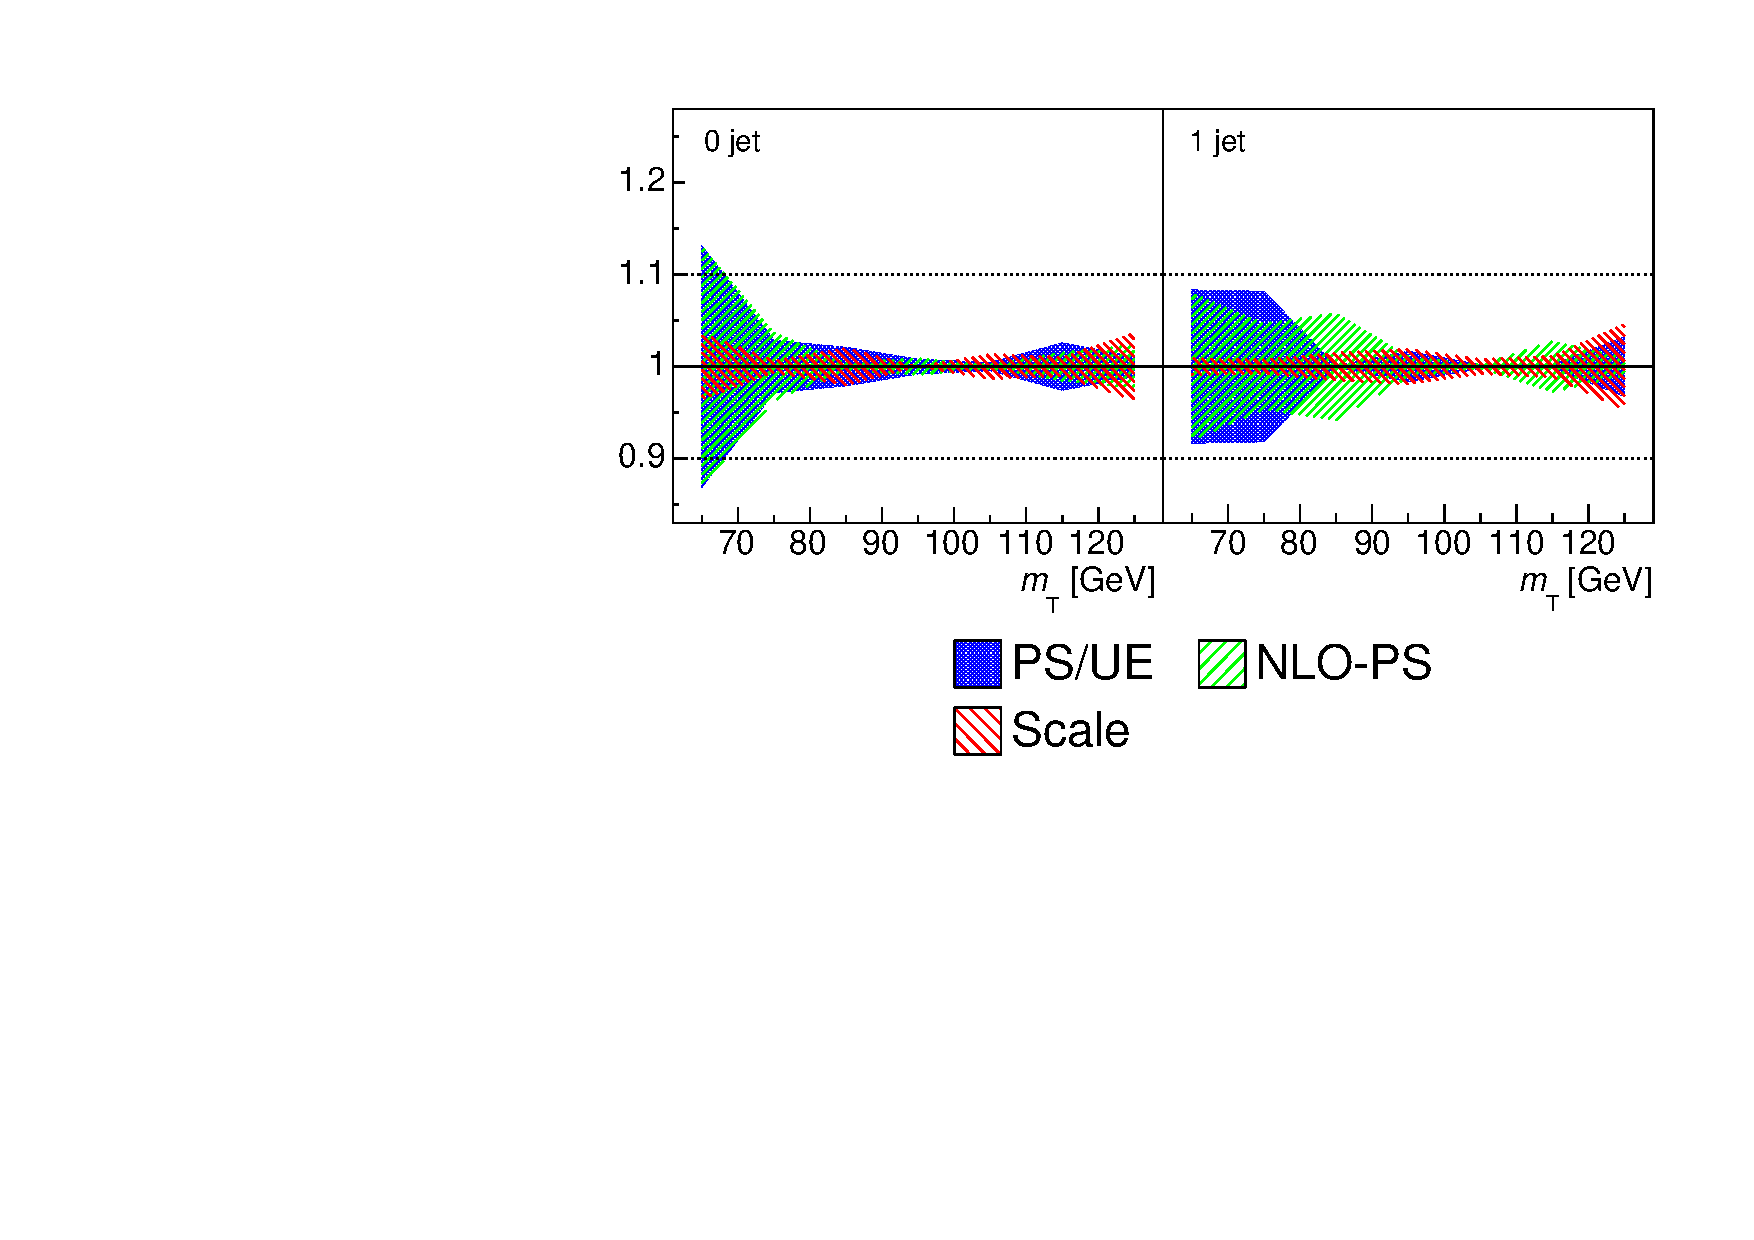
\includegraphics[width=\hugefigwidth]{custom_images/mT-shapes/ggf}
	\caption{ggF \mt shape systematic uncertainties in the 0-jet and 1-jet signal regions 
	of the \emch/\mech channels.}
	\label{fig:signal:mTshape}
\end{figure}


\subsection{ME-PS matching}
\label{sec:ggF:meps_matching}

When studying the uncertainties described above, a discrepancy was observed at high jet 
multiplicity between \meps{\powhegbox}{\pythia{8}} and \meps{\powhegbox}{\pythia{6}} (see 
green and black lines in \Figure~\ref{fig:signal:matching}). Its effect is properly 
accounted for in the above uncertainties, but the discrepancy is interesting in itself.
It was also observed in other electroweak processes.

The hadronisation and UE models of standalone \pythia{8} have been tuned to ATLAS 
UE data with a variety of PDF sets (known as AU2 tunes) \cite{ATLAS:tune:2012}.
However, the parton shower was not tuned since the default settings gave good agreement. 

When modelling ggF with \powhegbox, the AU2-CT10 tune was used in order to match the 
PDFs used in the matrix element calculation. Technically speaking, a dedicated 
\meps{\powhegbox}{\pythia{8}} tune should have been used, but this was unavailable. 
Unfortunately, a couple of issues had a negative impact on the NLO-PS matching. First, 
the parton shower evolves \alphaS at LO while NLO PDFs were used in the shower. 
Second, there was a mismatch between the \alphaS used in \powhegbox, 
$\alphaS\parenths{\mZ} = 0.118$, and the default value in the parton shower, 
$\alphaS\parenths{\mZ} = 0.137$. The effect of these issues is shown in 
\Figure~\ref{fig:signal:matching}.

\begin{figure}
	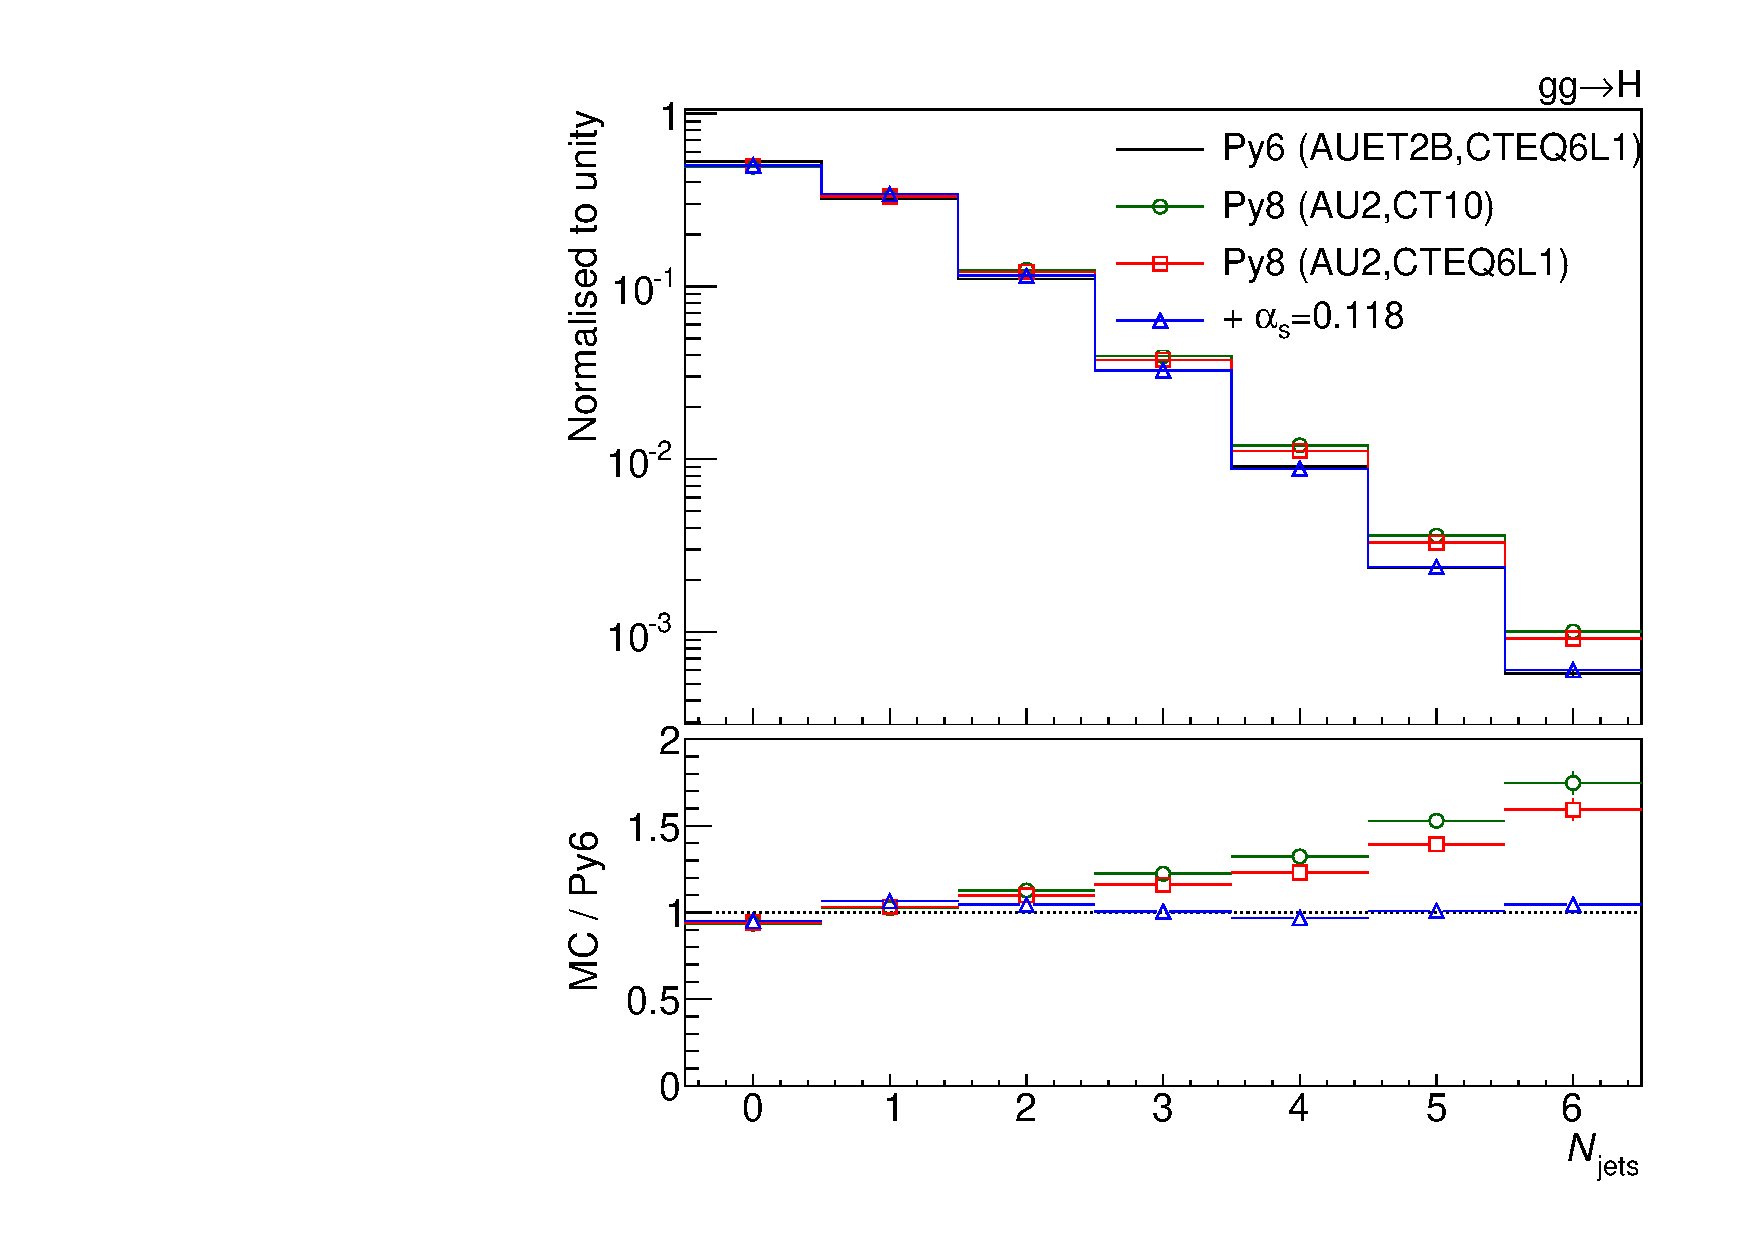
\includegraphics[width=\smallfigwidth]{tex/signal/matching}
	\caption{Jet multiplicity produced by \meps{\powhegbox}{\pythia{8}} with a selection 
	of shower tunes. The green circles is the tune used in the analysis. The red squares 
	change the parton shower PDFs from CT10 to CTEQ6L1. The blue triangles additionally 
	change the parton shower $\alphaS\parenths{\mZ}$ from 0.137 to 0.118 (in agreement 
	with \powhegbox). \meps{\powhegbox}{\pythia{6}} is shown in black for reference.}
	\label{fig:signal:matching}
\end{figure}

Identification of this poor matching has led to improvements in the latest round of MC 
tuning, where dedicated \meps{\powhegbox}{\pythia{8}} tunes are fit using an adjusted 
parton shower \cite{ATLAS:tune:2013}.
